\chapter{\textsl{Hilbert Space}}

本章的叙述思路为

\section{由内积生成范数}

\begin{mdframed}
    \begin{lemma}
        (\textbf{Schwarz不等式})  $\left| (x,y) \right|^2\leqslant (x,x)(y,y)$
    \end{lemma}
\end{mdframed}

\textbf{proof.} 该证明是构造性的方法,思路是想办法构造出$\left|(x,y)\right|^2$和$(x,x),(y,y)$的关系。取任意$\lambda\in \mathbb{C}$,$x,y\in \mathcal{H}$都满足

\begin{equation}
    (x+\lambda y,x+\lambda y)=(x,x)+\lambda(x,y)+\overline{\lambda}(x,y)+|\lambda|^2(y,y)\geqslant 0
\end{equation}

由$\lambda$的任意性,取$\lambda=-\displaystyle\frac{(x,y)}{(y,y)}$
\begin{equation}
    (x,x)-2\displaystyle\frac{|(x,y)|^2}{(y,y)}+\displaystyle\frac{|(x,y)|^2}{(y,y)}\geqslant 0
\end{equation}

稍微移项就可以得到结论。 $\Box$

\begin{mdframed}
    \begin{theorem}
        内积诱导\textsl{内积空间}上的范数
        \begin{equation}
            \Vert x\Vert=\sqrt{(x,x)}
        \end{equation}

        按照上面的范数,每个\textsl{内积空间}$\mathcal{H}$构成一个\textbf{赋范空间}。
    \end{theorem}
\end{mdframed}
 
\section{内积与范数之间的关系}

在内积可以诱导\textsl{Hilbert Space}上的范数,范数、和内积的关系在于:首先内积可以无条件诱导出范数,然后这些由内积诱导的范数可以通过一些特殊的构造诱导出内积(因为由内积诱导的范数必定满足平行四边形法则)。但内积并不等同于范数,因为有一类特殊的线性赋范空间存在,它存在范数,但这个范数不满足平行四边形公式,构造不出内积。

\begin{mdframed}
    \begin{lemma}
        $H$是内积空间,对于任意的$x,y\in H$
        \begin{enumerate}[itemindent=2em]
            \item \textbf{平行四边形法则}
            \begin{equation}
                \Vert x+y\Vert^2+\Vert x-y\Vert^2=2\Vert x\Vert^2+2\Vert y\Vert^2
            \end{equation}
            \item \textbf{极化恒等式}
            \begin{equation}
                (x,y)=\frac{1}{4}(\Vert x+y\Vert^2-\Vert x-y\Vert^2+i\Vert x+iy\Vert^2-i\Vert x-iy\Vert^2)
            \end{equation}
        \end{enumerate}
    \end{lemma}
\end{mdframed}
\textbf{proof.} 

$\Box$

平行四边形的几何意义为:\textsl{平行四边形对角线的平方和等于四条边的平方和}。这个结果是有点奇怪但是挺现实的,想像一下一个正方形,根据勾股定理很容易满足平行四边形法则,问题是你会发现任意的平行四边形都可用一个正方形改变角度得到。
\begin{figure}[H]
    \centering
    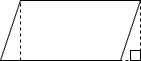
\includegraphics[scale=0.8]{figures/平行四边形法则.png}
    \caption{我可以抓着矩形一条边,平行拉动,这就变成了平行四边形,只不过角度变了}
\end{figure}
\begin{mdframed}
    \begin{theorem}
        设$X$是一个赋范空间,如果范数满足平行四边形法则,则可以在$X$中定义一个内积,使得由这个内积产生的范数正好是$X$原来的范数。
    \end{theorem}
\end{mdframed}
\textbf{proof.} 这个问题在于:\textbf{怎么利用范数去构造一个双线性函数,使得这个双线性函数满足的定义。}

$\Box$

本节的主定理告诉我们:当这个赋范空间上的范数满足平行四边形法则,才能定义其上的一个内积。

\section{完备的内积空间—\textsl{Hilbert Space}}

当内积空间中每一个\textsl{Cauchy sequence}都收敛,即满足完备性,我们称这样的空间为\textbf{\textsl{Hilbert Space}}。

\section{正交、正交补与正交分解}

对于内积我们自然关心其正交性,如果两个向量$x,y\in\mathcal{H}$,如果满足$(x,y)=0$,我们称之为\textbf{\textsl{正交}}。如果$M,N\subset \mathcal{H}$,对于$\forall x\in M,y\in N$,都有$(x,y)=0$,则我们称这两个\textbf{集合正交}。

下面我们定义所谓\textbf{\textsl{正交补空间}},设$X$是\textsl{Hilbert}空间,$M$是$X$子集,$M$的正交补空间定义为
\begin{equation}
    M^{\perp}=\{\ x\in X\ |\ (x,y)=0,\forall\ y\in M\ \}
\end{equation}

正交补有如下的性质,比较直观因此不作证明
\begin{enumerate}[itemindent=2em]
    \item $0\in M^\perp$;
    \item 如果$0\in M$,则$M\cap M^\perp=\{0\}$,否则$M\cap M^\perp=\emptyset$;
    \item $\{0\}^\perp=X$,$X\perp=\{0\}$;
    \item 如果$B(a,r)\subset M$,其中$B(a,r)$是以$a\in X$为中心,$r$为半径的开球,那么$M^\perp=\{0\}$,更进一步,如果$M$是一个非空的开集,则$M^\perp=\{0\}$;
    \item 如果$N\subset M$,那么$M^\perp \subset N^\perp$;
    \item $M\subset (M^\perp)^\perp$;
\end{enumerate}

本节主要定理有两个
\begin{mdframed}
    \begin{theorem}
        设$X$是内积空间,$M$是$X$的任意子集,则$M^\perp$是$X$中闭子空间;
    \end{theorem}
\end{mdframed}
\textbf{proof.}$\Box$

\begin{mdframed}
    \begin{theorem}
        设$M$是内积空间$X$的一个线性子空间,则$x\in M^\perp$当且仅当对于任意的$y\in M$,有$\Vert x-y\Vert \geqslant \Vert x\Vert$
    \end{theorem}
\end{mdframed}
\textbf{proof.}$\Box$

\section{最佳逼近}

\begin{mdframed}
    \begin{theorem}
        内积空间是严格凸的赋范空间。
    \end{theorem}
\end{mdframed}
\textbf{proof.}

\begin{mdframed}
    \begin{theorem}
        设$M$是\textsl{Hilbert}空间$\mathcal{H}$中的非空闭凸集,则对于任意$x\in \mathcal{H}$,存在唯一的最佳逼近点$x_0\in M$使得
        \begin{equation}
            \Vert x-x_0\Vert = d(x,M)=\inf\{\Vert x-y\Vert\ |\ y\in M\ \}
        \end{equation}
    \end{theorem}
\end{mdframed}
\textbf{proof.}

\section{\textsl{Hilbert}空间的正交分解定理}

三维的欧几里德空间可以分解为三个一维子空间的正交和(类似三维空间中的受力分解到$xyz$),我们把这一想法推广到一半的\textsl{Hilbert空间}。

\begin{mdframed}
    \begin{theorem}
        (\textbf{正交分解定理}) 设$\mathcal{H}$是\textsl{Hilbert空间},$M$是$\mathcal{H}$中的闭子空间,则对于任意的$x\in \mathcal{H}$,存在唯一的$x_0\in M$以及$y\in M^\perp$,使得
        \begin{equation}
            x=x_0+y
        \end{equation}

        并且
        \begin{equation}
            \Vert x\Vert^2=\Vert x_0\Vert^2+\Vert y\Vert^2
        \end{equation}
    \end{theorem}
\end{mdframed}

\textbf{proof.}

\section{正交系}

上面说的正交补空间是两个子集之间的元素相互正交,如果希尔伯特空间的一个子集$M$子集的元素之间相互正交,那么我们称$M$为\textbf{\textsl{正交系}},如果$M$中每一个元素的范数(由内积诱导的)都等于$1$,则我们称$M$为\textbf{\textsl{标准正交系}}

\subsection*{\textsl{正交系是线性无关的}}

\begin{mdframed}
    \begin{theorem}
        设$\{e_1,e_2,\cdots,e_k\}$是内积空间$X$中的正交系,则$\{e_1,e_2,\cdots,e_k\}$是线性无关的,如果$X$是$k$维的,且$\{e_1,e_2,\cdots,e_k\}$是标准正交系,则任何的$x\in X$都可以表示为
        \begin{equation}
            x=\sum\limits_{n=1}^{k}(x,e_n)e_n
        \end{equation}
    \end{theorem}
\end{mdframed}

\textbf{proof.}

\section{\textsl{Fouries Series}}

\section{正交基}

设$\{x_\alpha\}$是$X$中正交系,如果它长成的子空间的闭包是全空间$X$,那么我们称$\{x_\alpha\}$为\textbf{\textsl{正交基}}。

\section{可分的\textsl{Hilbert}空间}

\subsection*{\textsl{线性无关组的正交化算法}}

\begin{mdframed}
    \begin{theorem}
        设$\{x_n\}$是内积空间$\mathcal{H}$中的可数子集,则在$\mathcal{H}$中存在标准正交列$\{e_n\}$,使得$\{e_n\}$和$\{x_n\}$张成的子空间相同。
    \end{theorem}
\end{mdframed}

\textbf{proof.}

\subsection*{\textsl{可分的\textsl{Hilbert}空间与$l^2$等构同距}}
\begin{mdframed}
    \begin{theorem}
        设$\mathcal{H}$是一个\textsl{Hilbert}空间,则$\mathcal{H}$是可分的当且仅当$\mathcal{H}$中有至多可数的标准正交基$S$。
    \end{theorem}
\end{mdframed}